\documentclass[a4paper,12pt]{article}
\usepackage[utf8]{inputenc}
\usepackage[french]{babel}
\usepackage[T1]{fontenc}
\usepackage[top=2cm,bottom=2cm,left=2cm,right=2cm]{geometry}
\usepackage{graphicx}
\usepackage{wrapfig}
\usepackage{url}

\begin{document}

\begin{titlepage}
	\begin{center}
		\Large{Année universitaire 2016-2017}\\
		\Large{Université de Caen Basse-Normandie}\\[1cm]
		
		\huge{Rapport sur le premier semestre}\\
		\vspace{3cm}
		
		Alexis Carreau\\
		Thomas Lécluse\\
		Emma Mauger\\
		Théo Sarrazin\\
		
	\normalsize{\textit{ ~ L2 Informatique}}\\
		\medskip
		\vspace{2cm}
		
	\end{center}
\end{titlepage}

\tableofcontents
\newpage

\section{Introduction}

	\subsection{Présentation}
	Nous avons choisi de réaliser l'IDE (Integrated Developpement Environnement), car nous voulions créer un outil que nous pourrions utiliser par la suite. Ce sujet nous semblais donc intéressant à faire.
	
	Un IDE fournit des facilités au programmeur pour le développement logiciel. Il a pour but de maximiser la productivité du programmeur. Il contient généralement :
	\begin{itemize}
		\item un éditeur de texte, 
		\item un interpréteur, 
		\item un debugger,
		\item un compilateur,
		\item des options avancées comme la recherche de termes, l'autocomplétion, la coloration syntaxique...
	\end{itemize}
	
	\subsection{Objectifs}
	
	Nous devons d'ici à la fin de l'année réaliser un IDE qui contiendra les éléments cités ci-dessus. Pour la coloration lexicale et l'analyse syntaxique du code nous utiliserons les programmes Lex et Yacc.
	
	\subsection{Déroulement et planning}
	
	Nous avons réparti équitablement le travail et le temps de travail de chacun. Malgré le fait que deux membres du groupe (Thomas et Théo) connaissaient déjà la bibliothèque graphique que l'on utilise et partaient donc avec un avantage non-négligeable. \\
	Les deux autres membres du groupe ont donc été aidés au début afin de leur expliquer les bases et de pouvoir démarrer sans trop de problèmes.\\
	
	Nous avons réparti les différentes tâches à effectuer pour le projet entre les membres du groupe. Certaines sont plus longues ou plus complexes, c'est pourquoi certains membres du groupe on une liste moins remplie que d'autres. Il ne faut donc pas se fier uniquement à cette liste.\\
	
	\begin{itemize}
		\item Alexis : Navigation / Gestion des projets
		\item Emma : Découpage en modules / Architecture projet / Recherche bibliographique / Barre de menu
		\item Théo : Coloration syntaxique / Analyse lexicale / Interface graphique / Gestion (sauvegarde, ouverture) des fichiers
		\item Thomas : Documentation / Interface graphique / Thème, apparence texte et fenêtre / Barre de status
		\item Tout le groupe : Rapports et présentation 
	\end{itemize}
	
\section{Détails techniques}

	\subsection{Bibliothèques utilisées}
	
	Nous avons choisi la bibliothèque graphique QT (version 4.8.7, prévue à la base pour le C++) ce pourquoi nous avons aussi eu besoin de Pyside (version 1.2.4), qui fait le lien vers le langage Python (version 3.4).\\
	
	La raison de ce choix est le fait que QT est un outil plus puissant de par sa richesse de fonctionnalités. Sa documentation est de plus très fournie car les utilisateurs de QT sont plus nombreux que ceux de Tkinter.
	
	\subsection{Techniques employées}
	
	Nous avons choisi un style de programmation orienté objet, puisque plus logique dans un projet de cette envergure. L'objet nous permet de mettre en application les notions vues en cours. Cela nous permet de personnaliser en ré-implémentant des classes de QT pour les adapter à nos besoins.\\
	
	Lex est un programme qui permet de reconaître des tokens qui sont des éléments d'une chaîne de caractères. Cela à l'aide de règles lexicales que l'on lui passe en entrée.\\
	Dans notre cas, nous utilisons Lex pour reconnaître les éléments que l'on écrit, afin de colorier ces derniers en fonction de leur rôle (identifiant, entier, déclaration...). On utilise également la sortie générée que l'on passe à un autre programme : Yacc.\\
	
	Yacc permet de générer un arbre syntaxique abstrait qui nous permet de vérifier que la syntaxe de notre code est correcte. Aussi, cela ne permet de proposer une complétion automatique en fonction de ce que l'on écrit.\\
	On doit également lui passer des règles, qui sont d'ordre grammaticales.
	
	\begin{figure}[h!]
		\begin{center}
			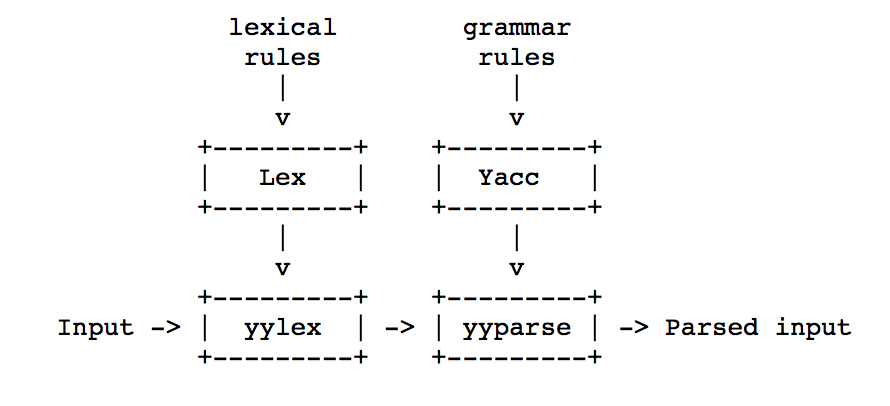
\includegraphics[scale=0.7]{images/schema_lex_yacc}
			\caption{Shéma résumant le foncionnement de Lex et Yacc.}
		\end{center}
	\end{figure}
	
	\subsection{Bibliographie}
	
	Nous avons utilisé deux sites de documentation principalement sur QT et Pyside.
	\begin{itemize}
		\item \url{http://srinikom.github.io/pyside-docs/PySide/QtGui/}
		\item \url{doc.qt.io}
	\end{itemize}
	
\section{Structure générale}

	\subsection{Répartition en modules}
	
		Les différents modules sont répartis par thèmes. Nous avons :
		\begin{itemize}
			\item Un module pour l'interface graphique
			\item Un module pour la gestion des projets
			\item Un module pour la gestion des fichiers
			\item Un module pour la coloration syntaxique
			\item Deux modules pour Lex et Yacc
			\item Un module pour l'analyse syntaxique
			\item Un module pour l'autocomplétion
		\end{itemize}
	
	\subsection{Module graphique}
	
		On retrouve dans ce module tout ce qui est relatif au GUI (l'interface graphique).\\
		C'est là qu'est créée la fenêtre principale de l'application. Où l'on va pouvoir créer, ouvrir, sauvegarder des fichiers et des projets.\\
		
		On y retrouve donc ce qui est nécessaire pour :
		
		\begin{itemize}
		
			\item Créer une zone de texte. Nous utilisons pour cela l'objet QTextEdit de QT, qui est un widget permettant d'avoir une zone de texte. Nous nous en servons comme fenêtre d'éditeur, c'est donc ici que l'on pourra coder.\\
			Le thème de l'application, c'est à dire la couleur de fond et de la police ainsi que la police utilisée sont relatif au QTextEdit. C'est également là que la couleur des élément (tokens) sera modifiée par Lex en fonction de leur rôle.\\
			\begin{center}
				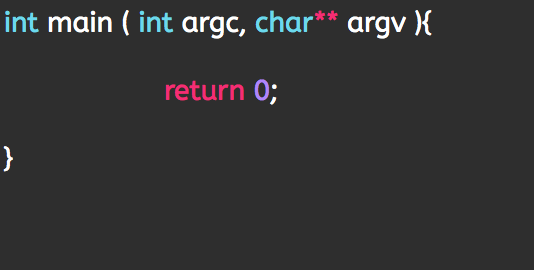
\includegraphics[scale=1]{images/QTextEdit}
				\vspace{0.5cm}
			\end{center}
			
			\item Créer plusieurs onglets de code. C'est un QTabWidget que nous utilisons pour cela, il va en fait créer plusieurs QTextEdit (ou en supprimer si on ferme l'onglet), et possède des fonctions et raccourcis pour naviguer entre tous. \\
			Si on a aucun onglet d'ouvert, on a le logo de notre groupe qui est affiché à la place.\\
			\begin{center}
				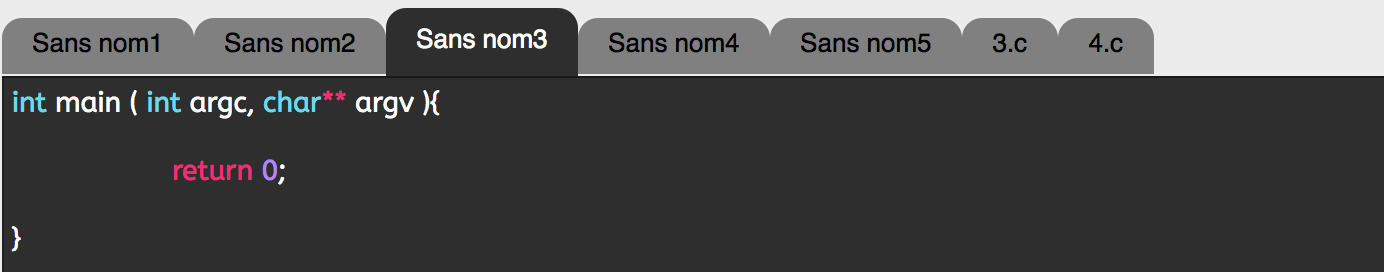
\includegraphics[scale=0.6]{images/QTabWidget}
				\vspace{0.5cm}
			\end{center}
			
			\item Créer une barre de menu. Cela permet d'avoir toutes les fonctionnalités et éventuellement des raccourcis. On utilise une QMenuBar pour cela, qui va elle-même utiliser une QAction pour créer une action sur le menu. Une action contient un nom, éventuellement un raccourci et une fonction à exécuter. 
			\begin{center}
				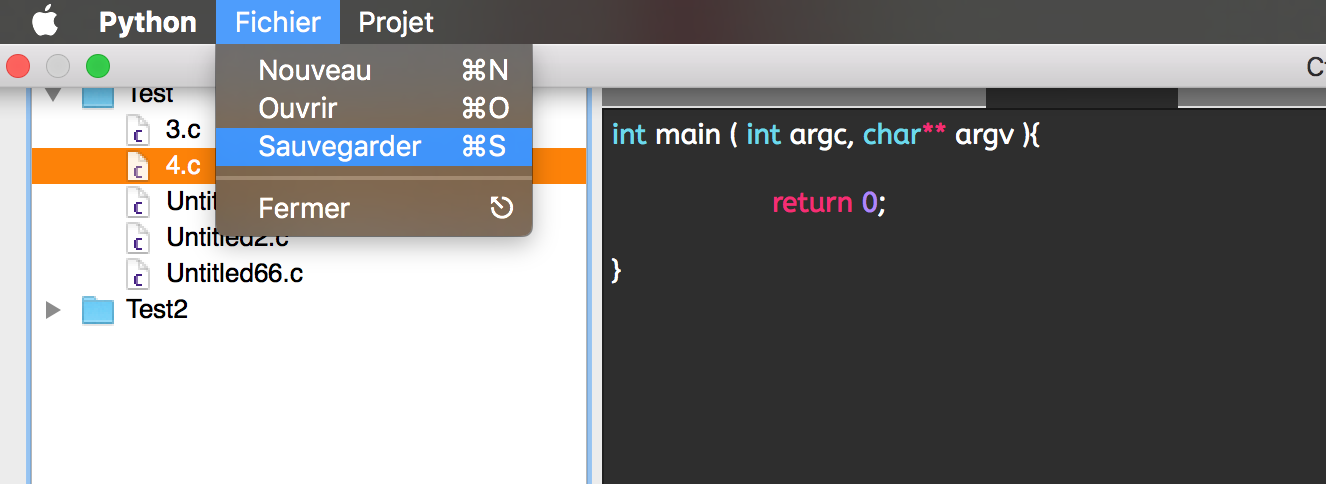
\includegraphics[scale=0.6]{images/QMenuBar}
				\vspace{0.5cm}
			\end{center}
			
			\item Mettre en place le navigateur de fichiers et de projets. On utilise un QTreeView qui nous permet d'afficher l'arborescence des fichiers et projets. C'est ce que l'on utilise pour ouvrir et naviguer dans les projets ouverts.\\
			\begin{center}
				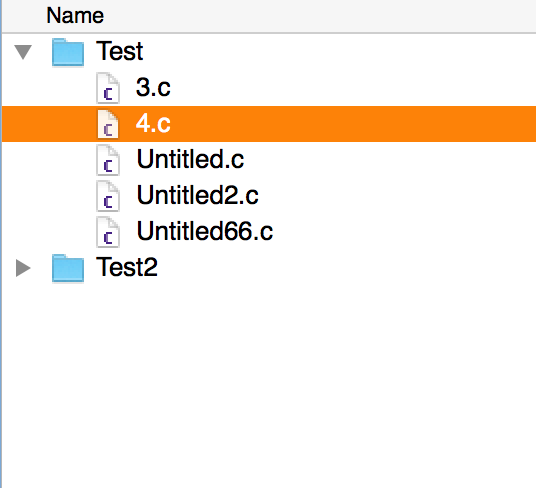
\includegraphics[scale=0.6]{images/QTreeView}
				\vspace{0.6cm}
			\end{center}
			
			\item Modifier la taille du navigateur de fichier/de l'éditeur de code. Pour cela, on utilise un QSplitter.\\ 
			Cela peut permettre, en fonction de la taille du projet et des répertoires imbriqués dans d'autres, de visualiser complètement les fichiers. Au on contraire, masquer le navigateur de fichier pour avoir une zone de code plus grande.\\
			
			\begin{center}
				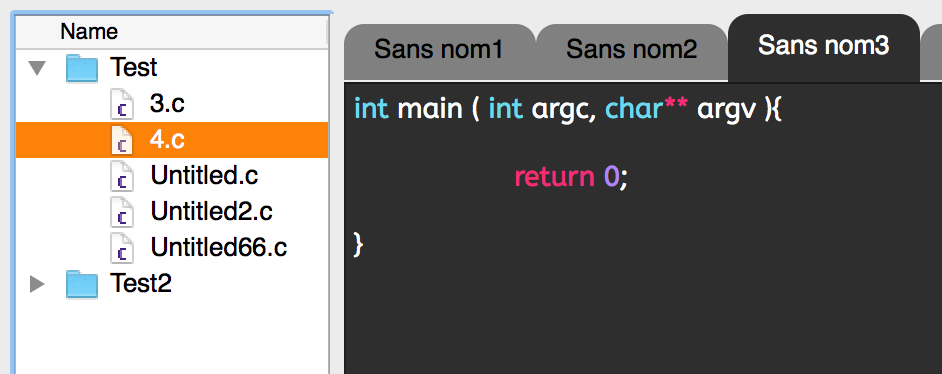
\includegraphics[scale=0.6]{images/QSplitter_1}
				\vspace{0.6cm}
			\end{center}

			\begin{center}
				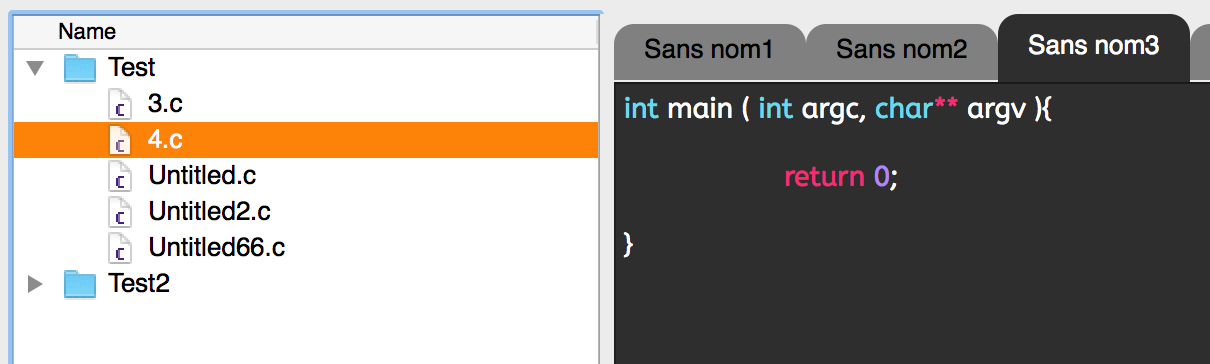
\includegraphics[scale=0.6]{images/QSplitter_2}
				\vspace{0.6cm}
			\end{center}
			
			\item Créer la fenêtre principale. On utilise un QWidget, qui est en fait une sorte de parent de tous les objets cités ci-dessus. C'est donc ici que l'on regroupe tout pour mettre en commun afin de faire un affichage propre.
			\begin{center}
				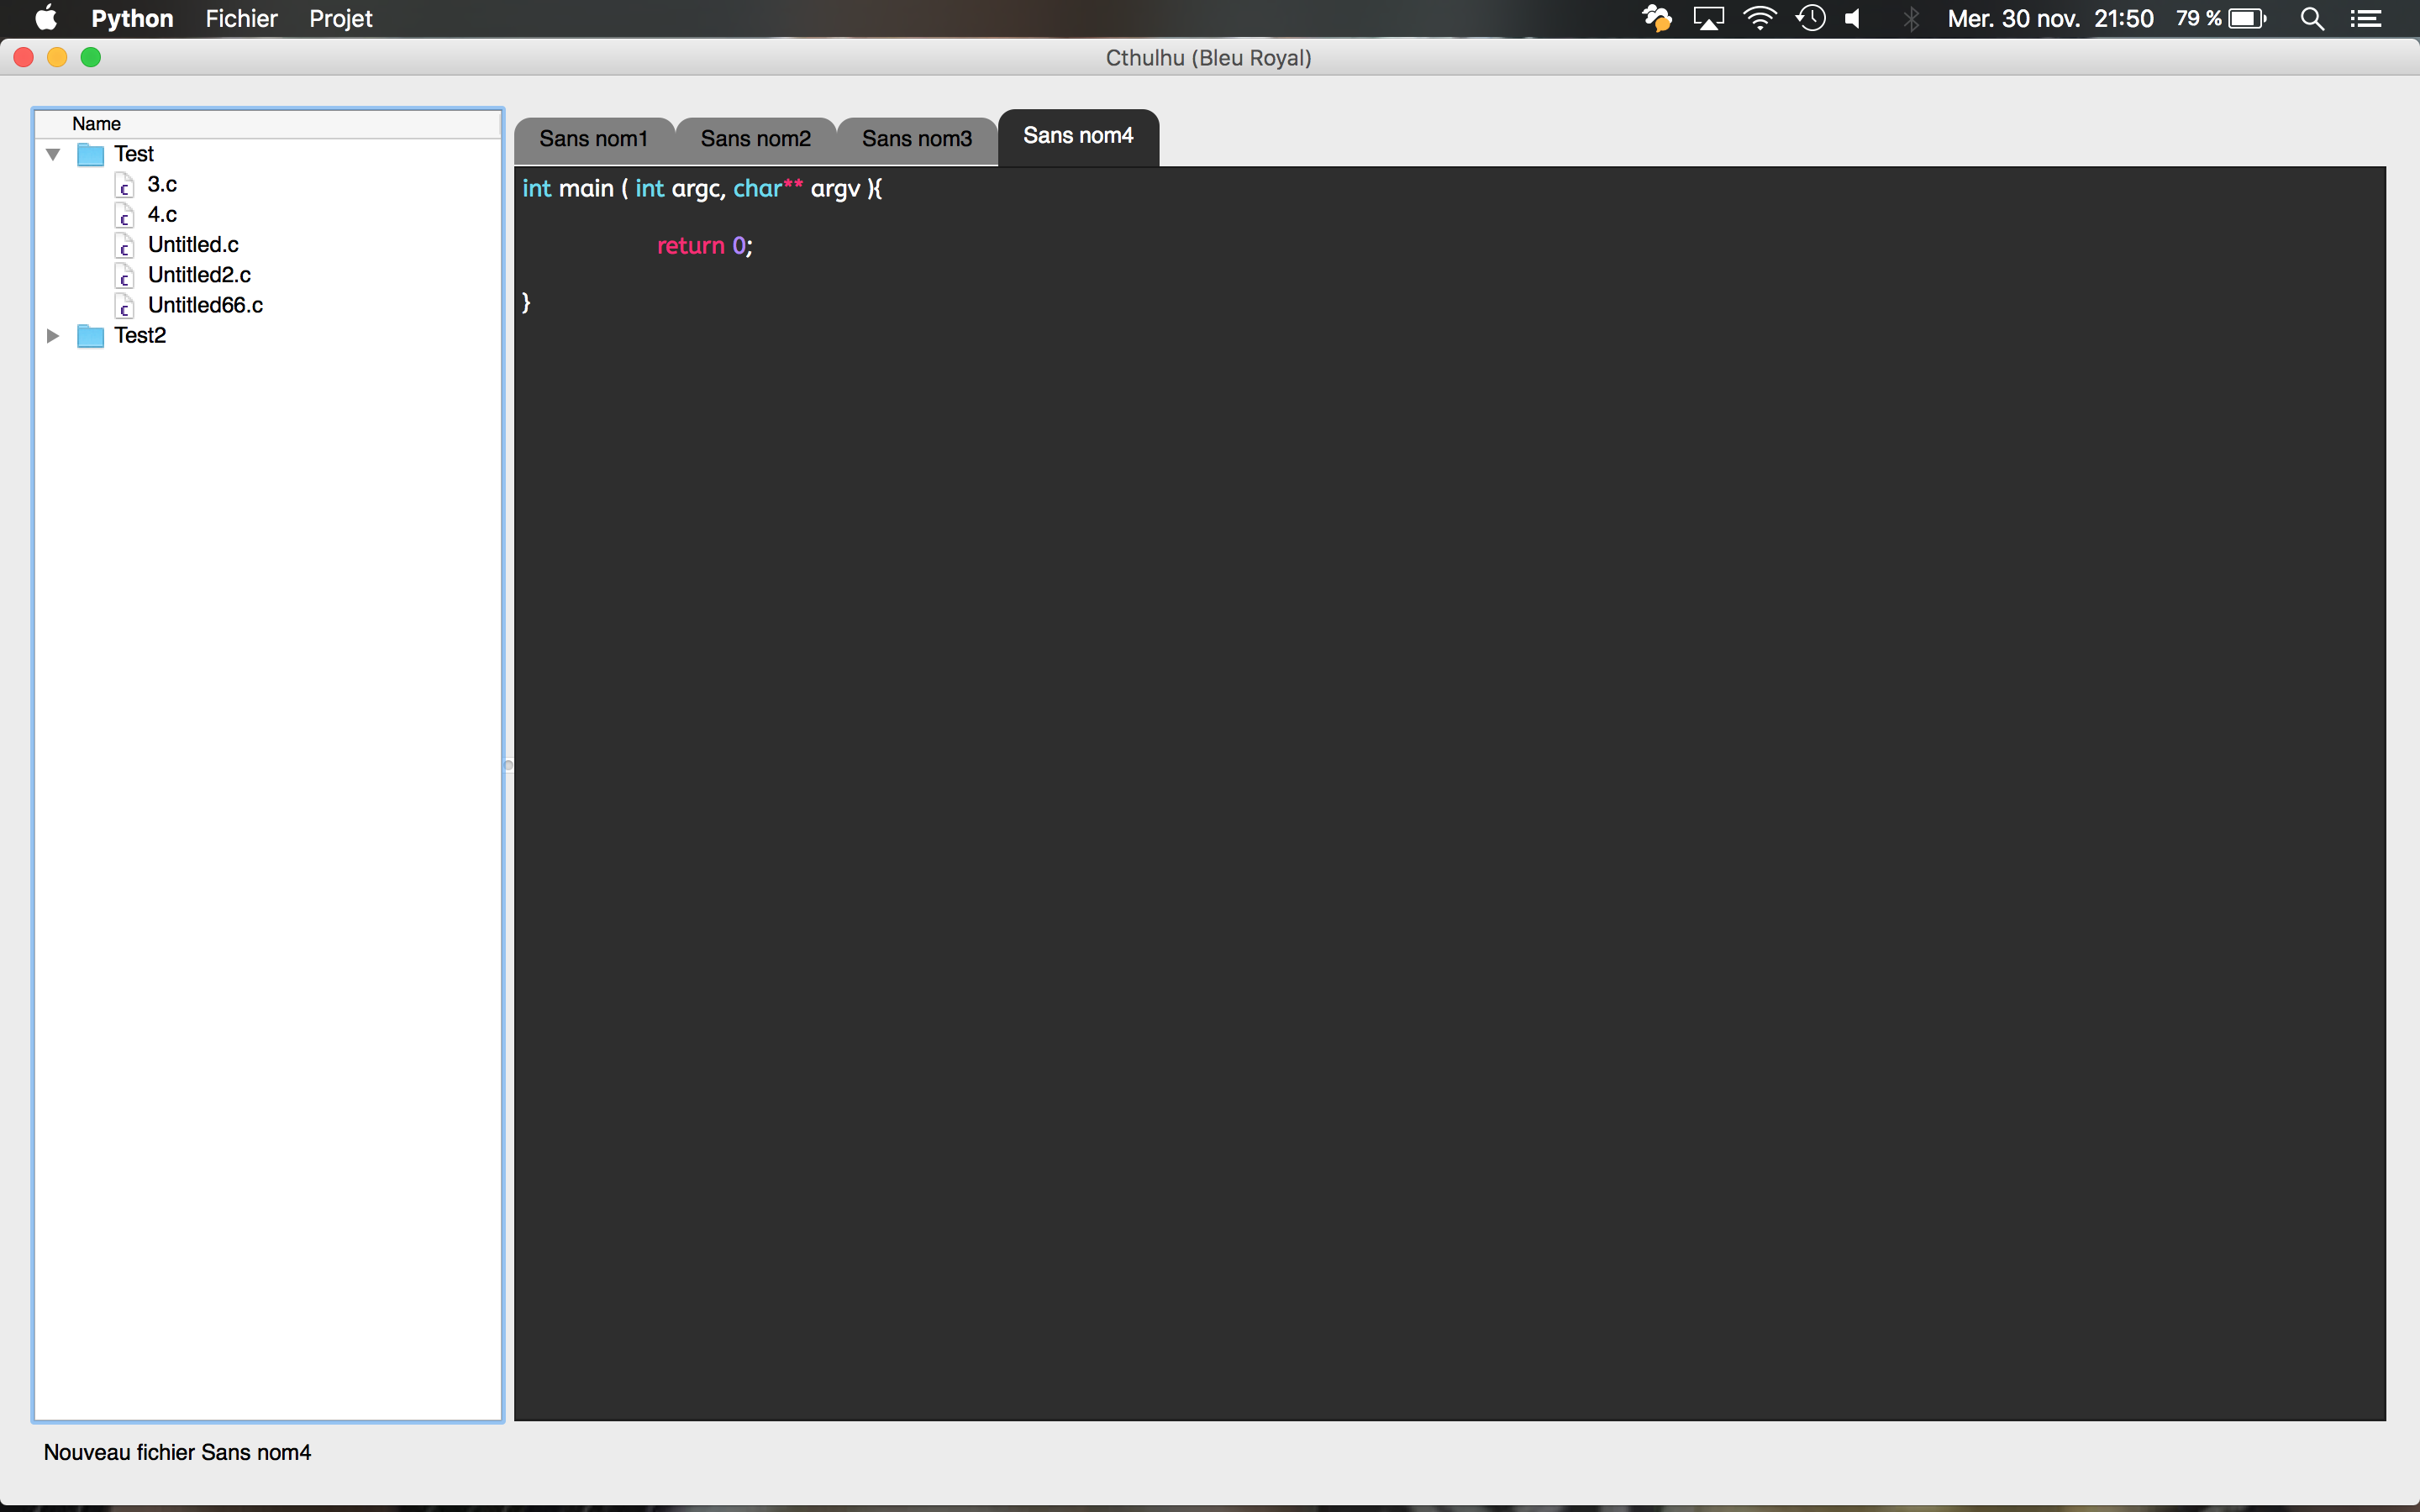
\includegraphics[scale=0.3]{images/QWidget}
				\vspace{0.6cm}
			\end{center}
			
		\end{itemize}
		
		Ce module est le plus imposant car la création d'un interface grafique nécessite beaucoup de lignes de codes.
		
		\subsection{Module gestion de projets}
			--> Déplacer les fonctions relatives dans un autre module que GUI
			
		\subsection{Module gestion de fichiers}	
	
\section{Conclusion}
	
	\subsection{Améliorations}

\end{document}